%!TEX root = ../thesis.tex

% \section{提案手法における従来の実験}

% \begin{itemize}
  \section{実験目的}
  シミュレータ上と実環境で, 提案手法の有効性の検証を行う
  \section{実験装置}
  % 4.1.1で述べた簡易的なシミュレータ環境とロボットで実験を行った
 \subsection{コンピュータとシミュレータ}
    \begin{enumerate}
      \item コンピュータ\\
      OS: Ubuntu 20.04 LTS\\
      ROS: Noetic\\
      CPU: intel Core i7-10700F(4.8GHz/8コア/16スレッド)\\
      DRAM: 32GB DDR4(3200/8GB×4)
      \item nav\_cloning(学習器, 統合環境)\\
      \url{https://github.com/open-rdc/nav_cloning}
      \item waypoint\_nav(移動目標地点, 目標方向を出力)\\
      \url{https://github.com/open-rdc/waypoint_nav}
      % \newpage
      \item turtlebot3 関連\\
      \url{https://github.com/open-rdc/turtlebot3}
      \newpage
      \item navigation(ナビゲーションパッケージ)\\
      \url{https://github.com/ros-planning/navigation}
    \end{enumerate}

    \subsection{ロボット}
    ロボットモデルは従来手法の検証に用いた実験\cite{okada1}\cite{okada2}と同様, \figref{Fig:waffle_pi}に示すような, TurtleBot3 Waffle\_pi\cite{turtlebot3}へ3つのカメラを追加したモデルを用いる.

    \begin{figure}[hbtp]
      \centering
    \includegraphics[keepaspectratio, scale=0.22]
          {images/Waffle_pi.png}
    \caption{TurtleBot3 waffle\_pi with 3 cameras}
    \label{Fig:waffle_pi}
    \end{figure}

    \subsection{環境}
    シミュレータ環境として, オープンソースの3DロボットシミュレータGazebo\cite{gazebo}を用いる. \figref{Fig:sim}に示すようなGazebo上で千葉工業大学津田沼キャンパス2号館3階を模した実験環境を対象に実験を行う.

    \begin{figure}[hbtp]
      \centering
    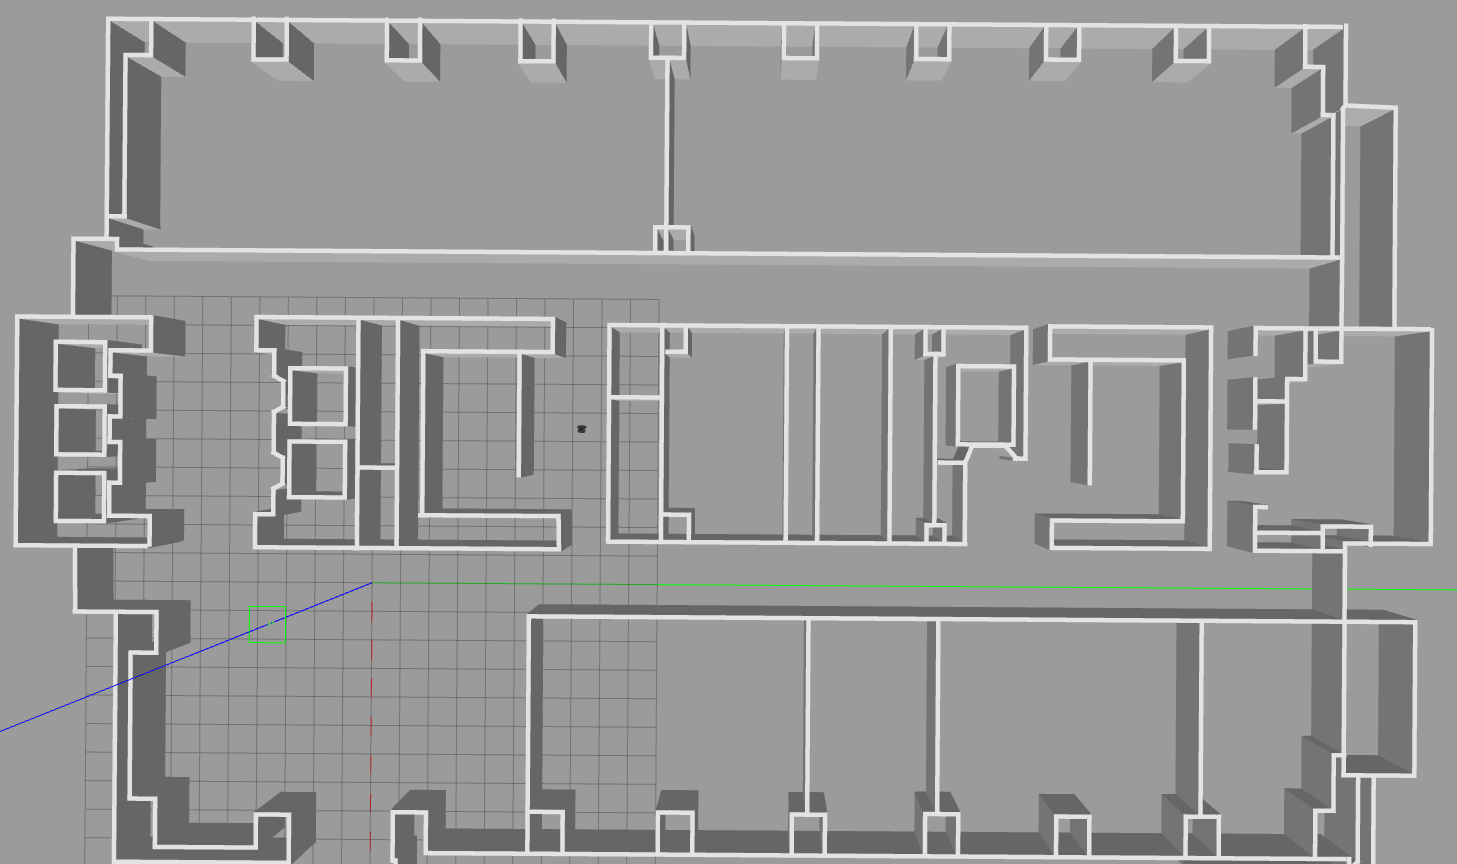
\includegraphics[keepaspectratio, scale=0.12]
          {images/tsudanuma2-3_simorg.png}
    \caption{Experimental environment of simulator}
    \label{Fig:sim}
    \end{figure}

  % \end{itemize}

  \section{実験方法}
  \figref{Fig:sim_explain}のA, B地点において, \figref{Fig:select}に示すように侵入する方向が3つあり, 進むことのできる方向が2つあることから, 1箇所につき走行パターンが6つ存在する. 
また, A, B地点では, 目標方向に従って任意の経路を選択することが求められる場所である.
したがって, 実験ではA, B地点で合計12パターンの走行において, 与えた目標方向に従った行動が行えるのかを確認する.

\begin{figure}[hbtp]
  \centering
 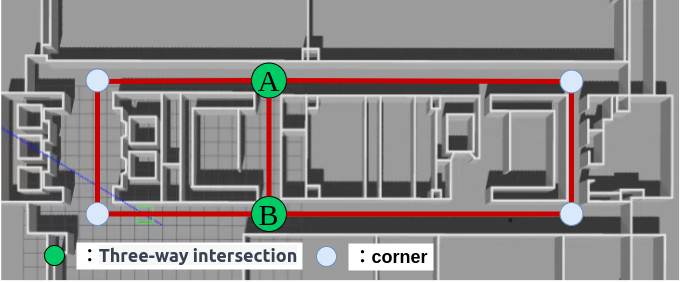
\includegraphics[keepaspectratio, scale=0.5]
      {images/sim_explain.png}
 \caption{Characteristics of passages in the experimental environment on the simulator}
 \label{Fig:sim_explain}
\end{figure}

\begin{figure}[hbtp]
  \centering
 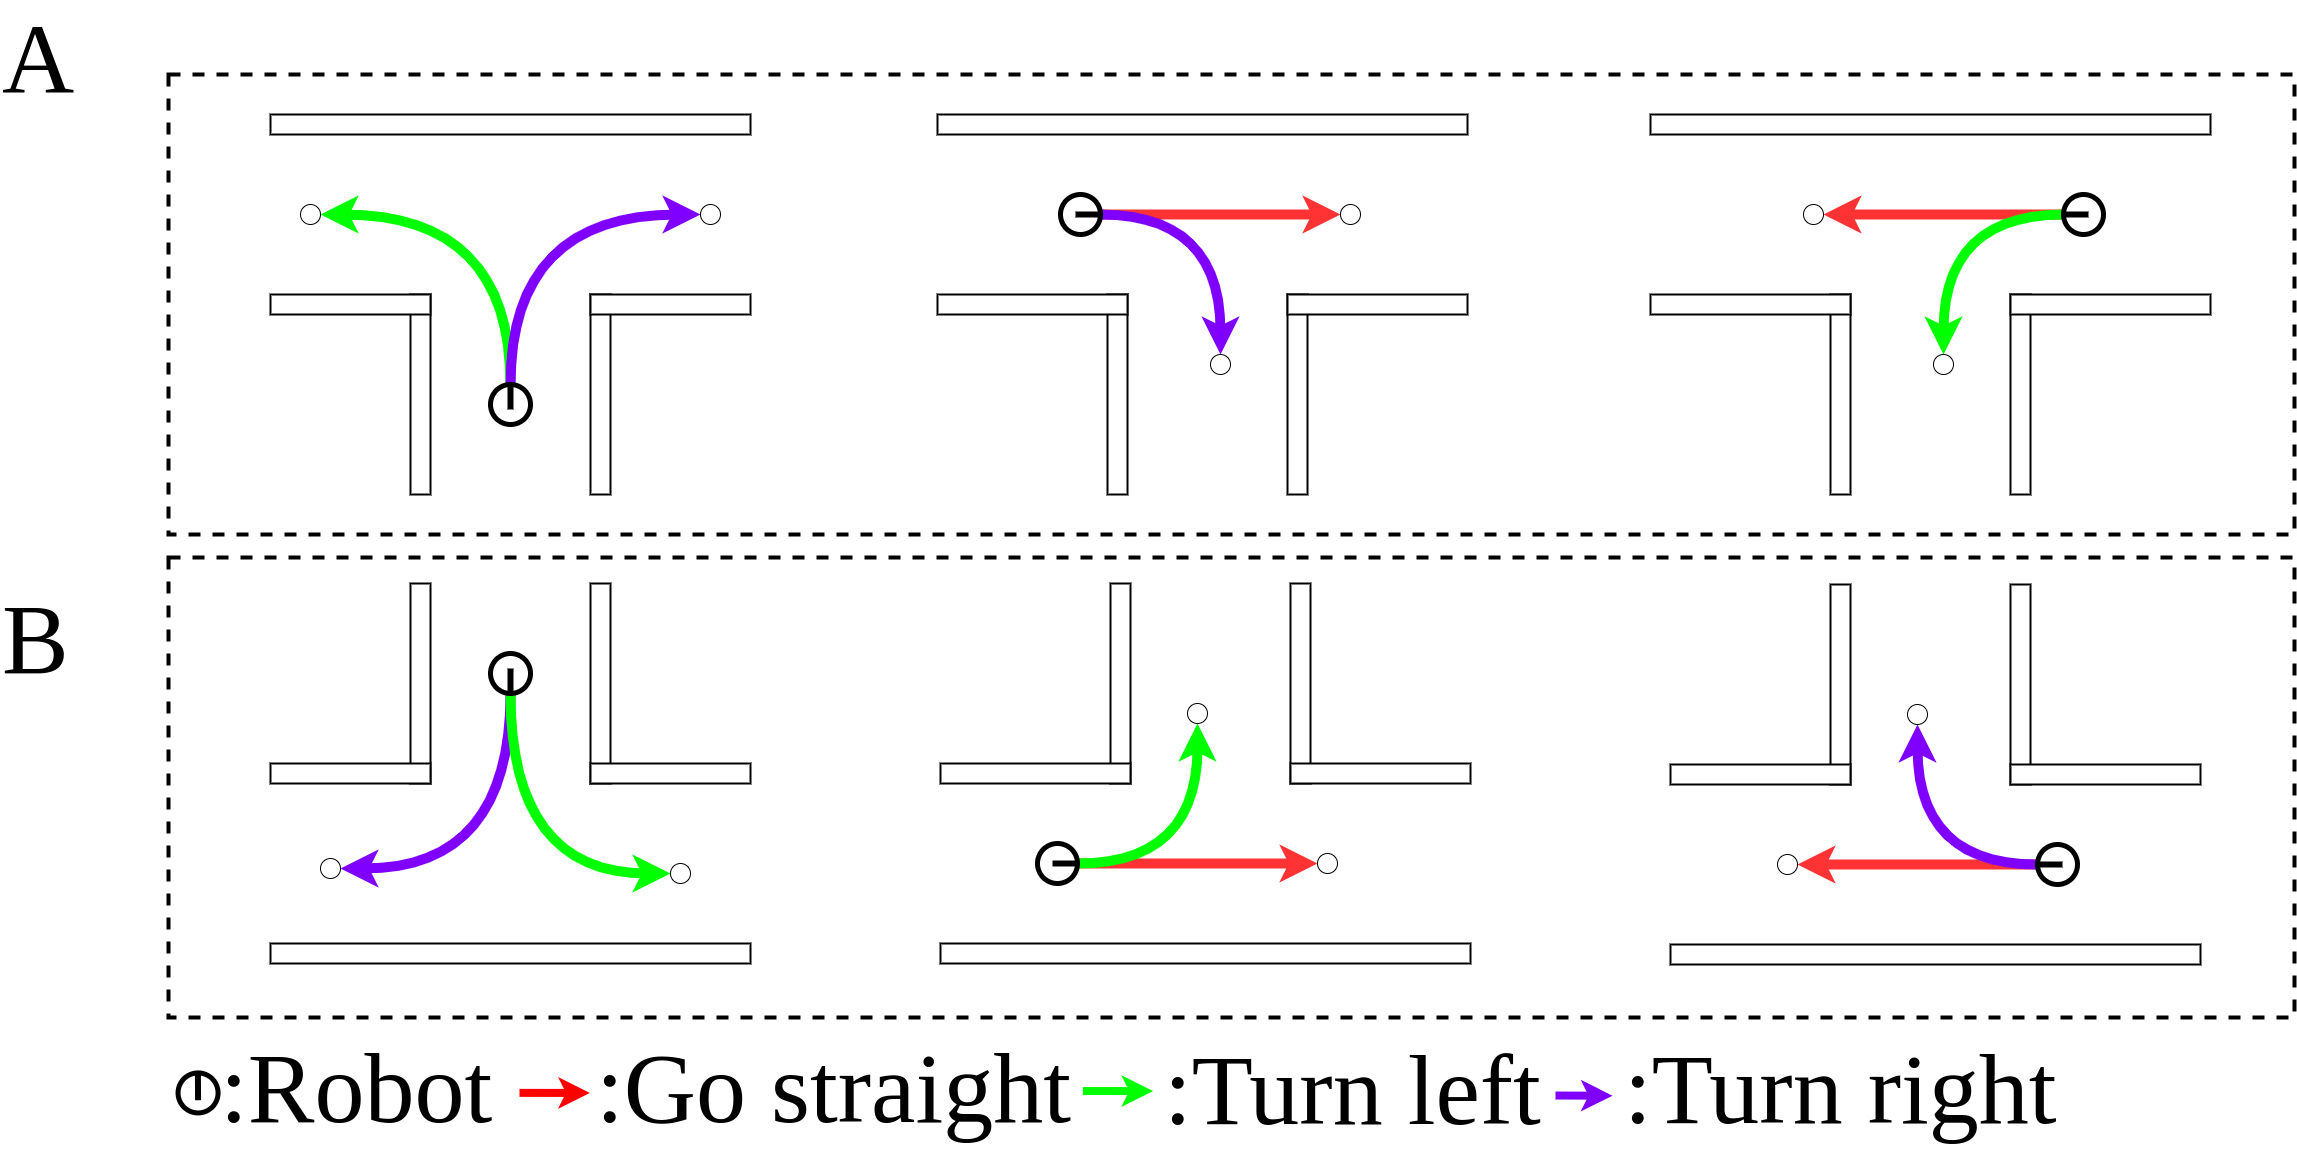
\includegraphics[keepaspectratio, scale=0.15]
      {images/select.png}
 \caption{Moving pattern at points A and B}
 \label{Fig:select}
\end{figure}

全ての走行パターンを網羅するように模倣学習を行うため, \figref{Fig:route}に示すようにaからfまでの経路を繰り返し走行させる. なお, 目標方向はwaypoint\_navから生成され, データセットに加えられる. 学習終了後, テストフェーズに移行するが, 学習時と同様にaからfまでの順番で経路をロボットに走行させる. また, テストフェーズ時にロボットが壁に衝突した場合, 経路の中央にロボットを移動させた後, 走行を再開させる.

\begin{figure}[hbtp]
  \centering
 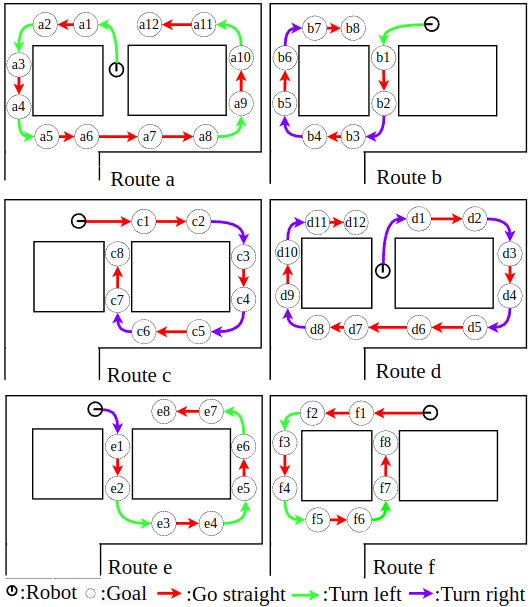
\includegraphics[keepaspectratio, scale=0.6]
      {images/route.png}
 \caption{The order of the route to be moved}
 \label{Fig:route}
\end{figure}

% \par
 学習を60000step実行後, テストフェーズに移行する. テストフェーズで正しい順序で経路を選択し, 走行を行えるか確認する. この一連の流れを10回繰り返し行う.

  % \newpage

  \section{実験結果}
  実験結果を\figref{Fig:60000step}に示す. この図は, それぞれの走行パターンにおいて正しく経路を選択し, 走行できた回数を表している. \tabref{table:result}に全パターンの成功回数を合計した結果を示す. なお, 分母が120であるのはテストフェーズにおいて, 全12パターンからなる経路を走行させ, 評価を行うことを10回繰り返したためである. 
  \par
  \tabref{table:result}に示すように, 目標方向に従って113/120回, 正しい経路を選択する様子が見られた. 成功率が約94\%となったことから, 簡易的なシミュレータ上では提案手法により, 経路を選択できることが判明した. しかし, \figref{Fig:60000step}のb3, e3に向かう選択ができていない. 特に, b3に関しては成功回数が著しく少ない. これは, \figref{Fig:howaie}に示すように, b3が評価対象である12パターンの中で, 唯一ホワイエに向かう経路であり, 他のパターンに比べて急激に取得するカメラ画像の特徴が変化することが影響したおそれがある. 
  % また, e3に関しては, 選択して向かう経路が他のパターンとほぼ同様の通路であるため, e3単体では失敗するとは考えにくい箇所である. このことから, b3に起因する失敗の可能性が高い.
  また, e3に関しては, カーブを行い始める段階で, 取得するカメラ画像にホワイエが写り込んでしまうことが影響したおそれがある.

% \vspace{2cm}

\begin{figure}[hbtp]
  \centering
 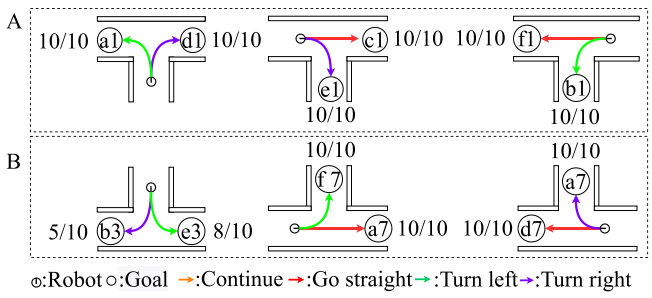
\includegraphics[keepaspectratio, scale=0.5]
      {images/60000step.png}
 \caption{Experimental results for each moving pattern from \cite{mech}}
 \label{Fig:60000step}
\end{figure}

% \vspace{1cm}
% \newpage

% \vspace{3cm}

\begin{table}[hbtp]
  \caption{Experimental results}
  \label{table:result}
  \centering
  \begin{tabular}{|c|c|}
    \hline
    Step & Total result\\
    \hline
    60000 & 113/120(94.2\%)\\
    \hline
  \end{tabular}
\end{table}

% \begin{figure}[h]
%   \centering
%   \begin{minipage}[b]{120mm}
%     \centering
%     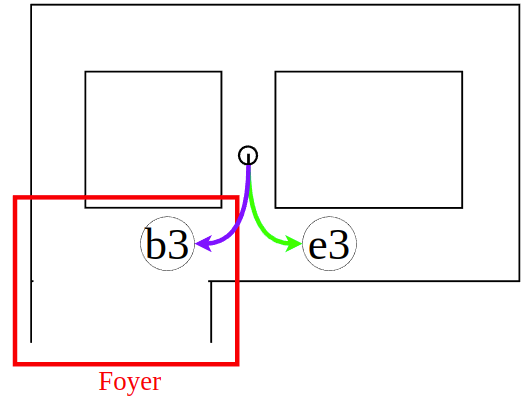
\includegraphics[keepaspectratio, scale=0.45]{images/howaie2.png}
%     \caption*{(a)}
%   \end{minipage} 
%   % \newpage
%   % \hspace{0.03\columnwidth}
%   \begin{minipage}[b]{120mm}
%     \centering
%     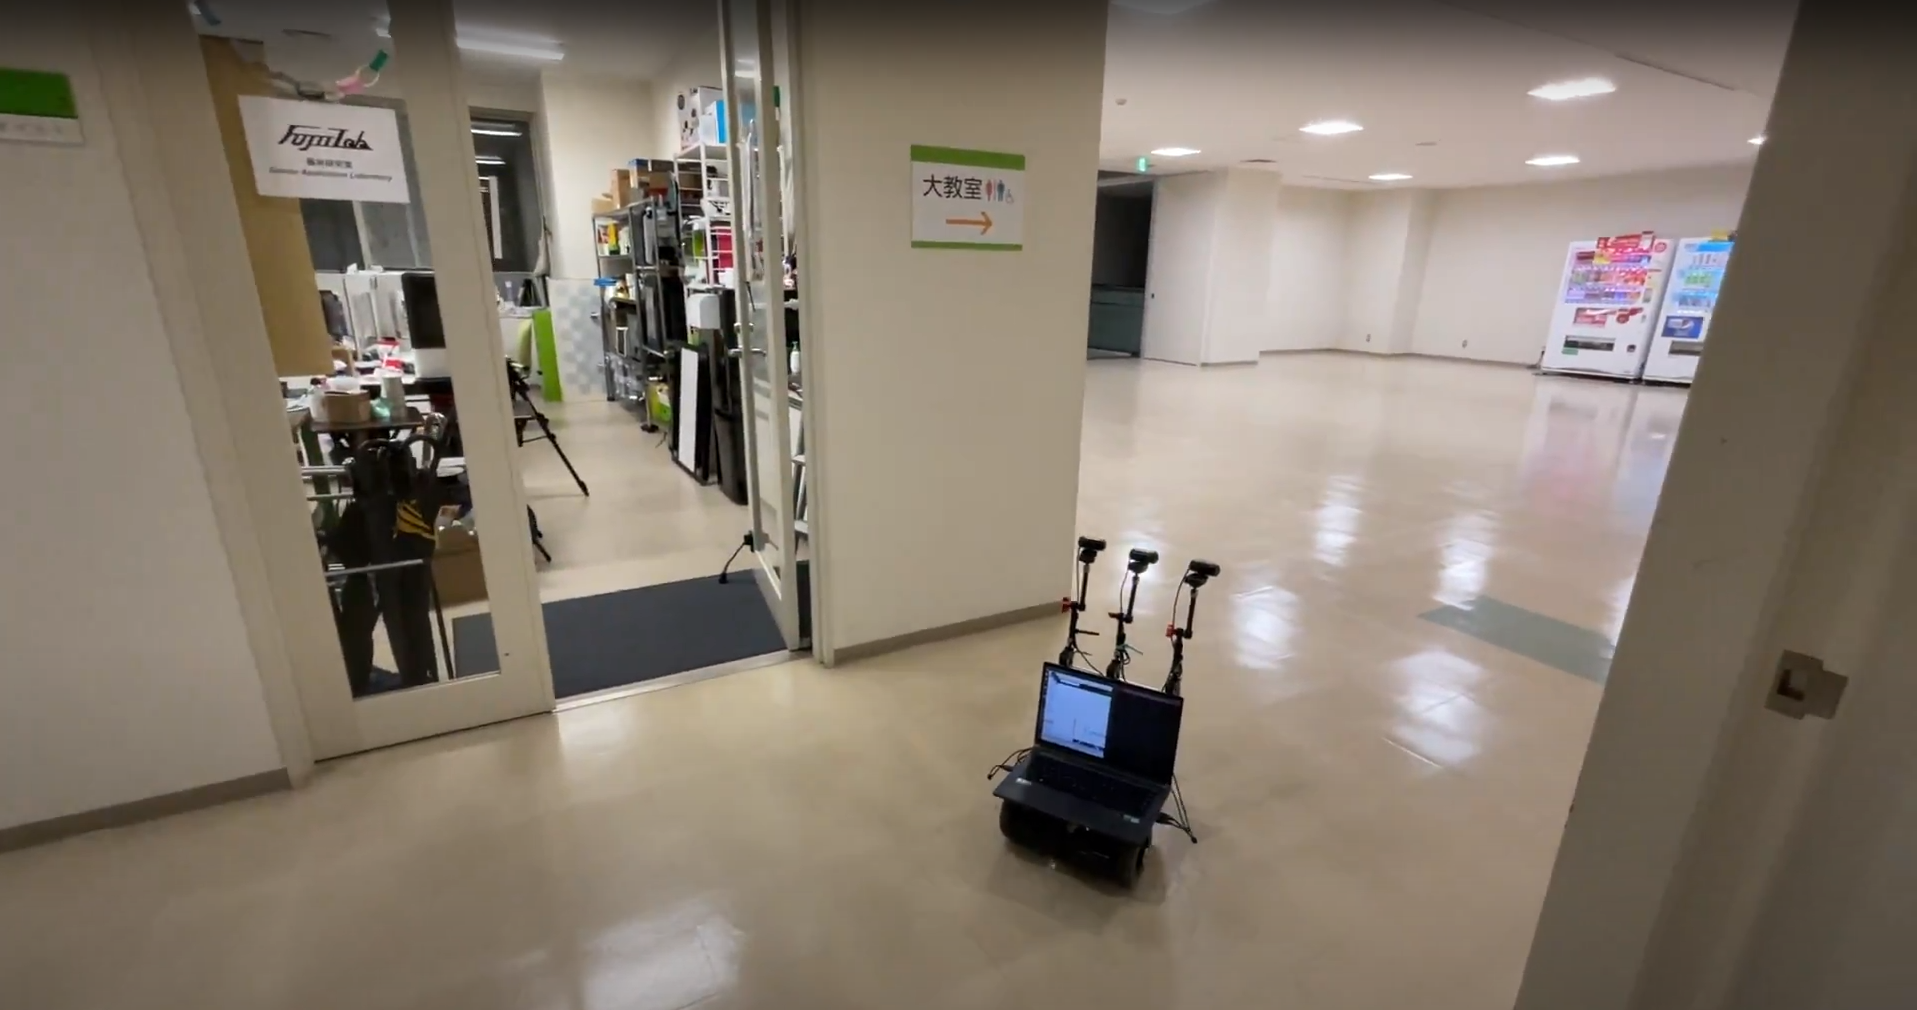
\includegraphics[keepaspectratio, scale=0.15]{images/example_howaie.png}
%     \caption*{(b)}
%   \end{minipage}
%   \caption{}
%   \label{Fig:howaie}
% \end{figure}

\begin{figure}[hbtp]
  \centering
 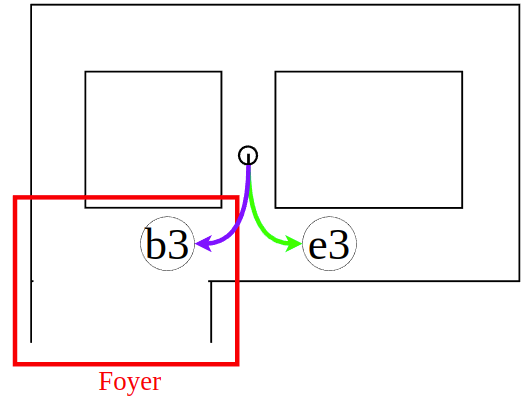
\includegraphics[keepaspectratio, scale=0.4]
      {images/howaie2.png}
 \caption{Foyer on the route to be moved}
 \label{Fig:howaie}
\end{figure}

次に, 実環境での実験を行った. 実験方法は, シミュレータ上での実験に倣って設定した. しかし, 実験を行ったのは1回のみである. 実験が1回のみなのは, 学習時間の長さが問題であったためである. 具体的には, 実験にはおよそ7時間を要し, バッテリなどの関係で1日に1, 2時間が限界であったため, 1週間かけて実験を行う必要があった. なお, 実験装置については後述する.

実験結果を \figref{Fig:60000step_real} に示す. この図は, それぞれの走行パターンにおいて正しく経路を選択し, 走行できた回数を表している. \tabref{table:result_real_60000} に実験ごとに全パターンの成功回数を合計した結果を示す. 表に示すように, 目標方向に従って 9/12 回, 正しい経路を選択する様子が見られた.

\begin{figure}[hbtp]
  \centering
 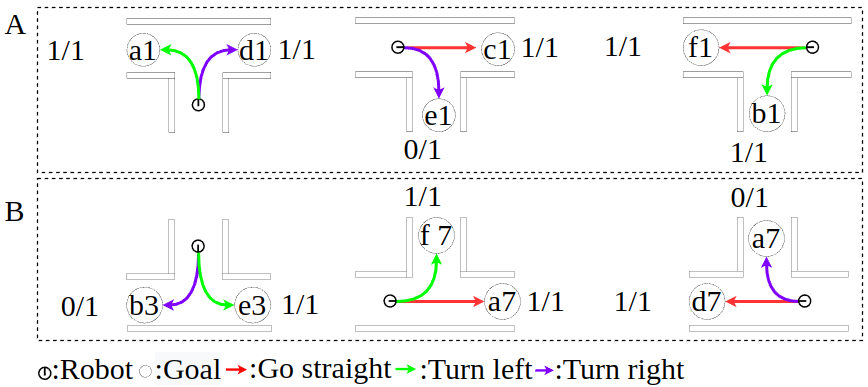
\includegraphics[keepaspectratio, scale=0.4]
      {images/60000step_real2.png}
 \caption{Experimental results for each moving pattern at 60000step by real environment}
 \label{Fig:60000step_real}
\end{figure}

\begin{table}[hbtp]
  \caption{Experimental results}
  \label{table:result_real_60000}
  \centering
  \begin{tabular}{|c|c|c|}
    \hline
    Experiments & Step & Total result\\
    \hline
    Simulator & 60000 & 113/120(94.2\%)\\
    \hline
    Real environment & 60000 & 9/12(75\%)\\
    \hline
  \end{tabular}
\end{table}

\tabref{table:result_real_60000}から, シミュレータ上と実環境で成功回数に大きく差があることがわかる. これについては, 5.6.4項で述べる.

% \end{itemize}
% \newpage

% \section{実環境での実験}
% \subsection{実験目的}
% 実環境で, 提案手法の有効性の検証を行う.
% \subsection{実験装置}
% \begin{itemize}
%   \item ロボット
  
%   ロボットは前報\cite{okada1}と同様, \figref{Fig:gamma}に示すように, 3つのカメラを搭載したロボットを用いる.

%   % \vspace{2cm}
  
%   \begin{figure}[hbtp]
%     \centering
%    \includegraphics[keepaspectratio, scale=0.45]
%         {images/gamma2.png}
%    \caption{Experimental setup from \cite{okada1}}
%    \label{Fig:gamma}
%   \end{figure}

%   % \newpage

%   \item 環境

%   \figref{Fig:real_environment}に示すような千葉工業大学津田沼キャンパス2号館3階で実験を行う.

%   \begin{figure}[h]
%     \centering
%     \begin{minipage}[b]{120mm}
%       \centering
%       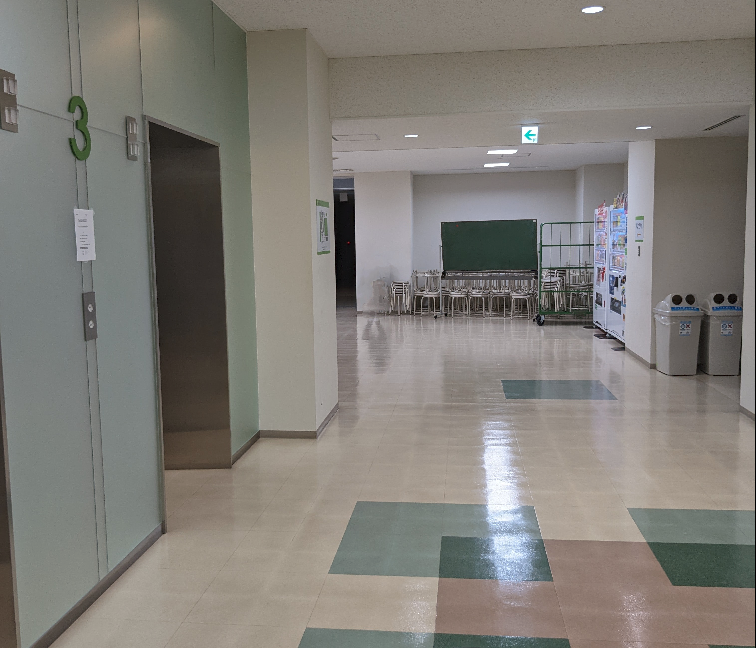
\includegraphics[width=40mm]{images/real.png}
%       \caption*{(a) One place in the real environment}
%     \end{minipage} 
%     % \newpage
%     % \hspace{0.03\columnwidth}
%     \begin{minipage}[b]{120mm}
%       \centering
%       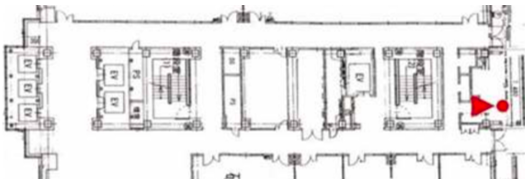
\includegraphics[width=95mm]{images/tsudanuma_structure.png}
%       \caption*{(b) structure}
%     \end{minipage}
%     \caption{Real environment}
%     \label{Fig:real_environment}
%   \end{figure}
% \end{itemize}

% \subsection{実験方法}
% シミュレータ上での実験に倣って設定した. しかし, 評価を行ったのは1回のみである.

% \newpage
% \subsection{実験結果}

% \begin{figure}[hbtp]
%   \centering
%  \includegraphics[keepaspectratio, scale=0.5]
%       {images/60000step_real.png}
%  \caption{Experimental results for each moving pattern from \cite{mech}}
%  \label{Fig:60000step_real}
% \end{figure}

\newpage